In Sections \ref{section:finite-diffences} -- \ref{section:continuous-adjoint} we focused on merely introducing each one of the sensitivity methods classified in Figure \ref{fig:scheme-all-methods} as separate methods, postponing the discussion about their points in common. 
In this section, we compare one-to-one these methods and highlight differences and parallels between them. 


\subsubsection{Forward AD and complex step differentiation}

Both AD based on dual numbers and complex-step differentiation introduce an abstract unit ($\epsilon$ and $i$, respectively) associated with the imaginary part of the dual variable that carries forward the numerical value of the gradient.
% This resemblance between the methods makes them susceptible to the same advantages and disadvantages: easiness of implementation with operator overloading; and inefficient scaling with respect to the number of variables to differentiate. 
Although these methods seem similar, AD gives the exact gradient value, whereas complex step differentiation relies on numerical approximations that are valid only when the stepsize $\varepsilon$ is small. 
In Figure \ref{fig:complex-step-AD} we show how the calculation of the gradient of the function $\sin (x^2)$ is performed by these two methods.
Whereas the second component of the dual number has the exact derivative of the function $\sin(x^2)$ with respect to $x$, it is not until we take $\varepsilon \rightarrow 0$ that we obtain the derivative in the imaginary component for the complex step method.
% The stepsize dependence of the complex step differentiation method makes it resemble more to finite differences than AD with dual numbers. 
The dependence of the complex step differentiation method on the step size gives it a closer resemblance to finite difference methods than to AD using dual numbers.
Further notice the complex step method involves more terms in the calculation, a consequence of the fact that second order terms of the form $i^2 = -1$ are transferred to the real part of the complex number, while for dual numbers the terms associated to $\epsilon^2 = 0$ vanish \cite{martins2001connection}. 

\begin{figure}[t]
    \centering
    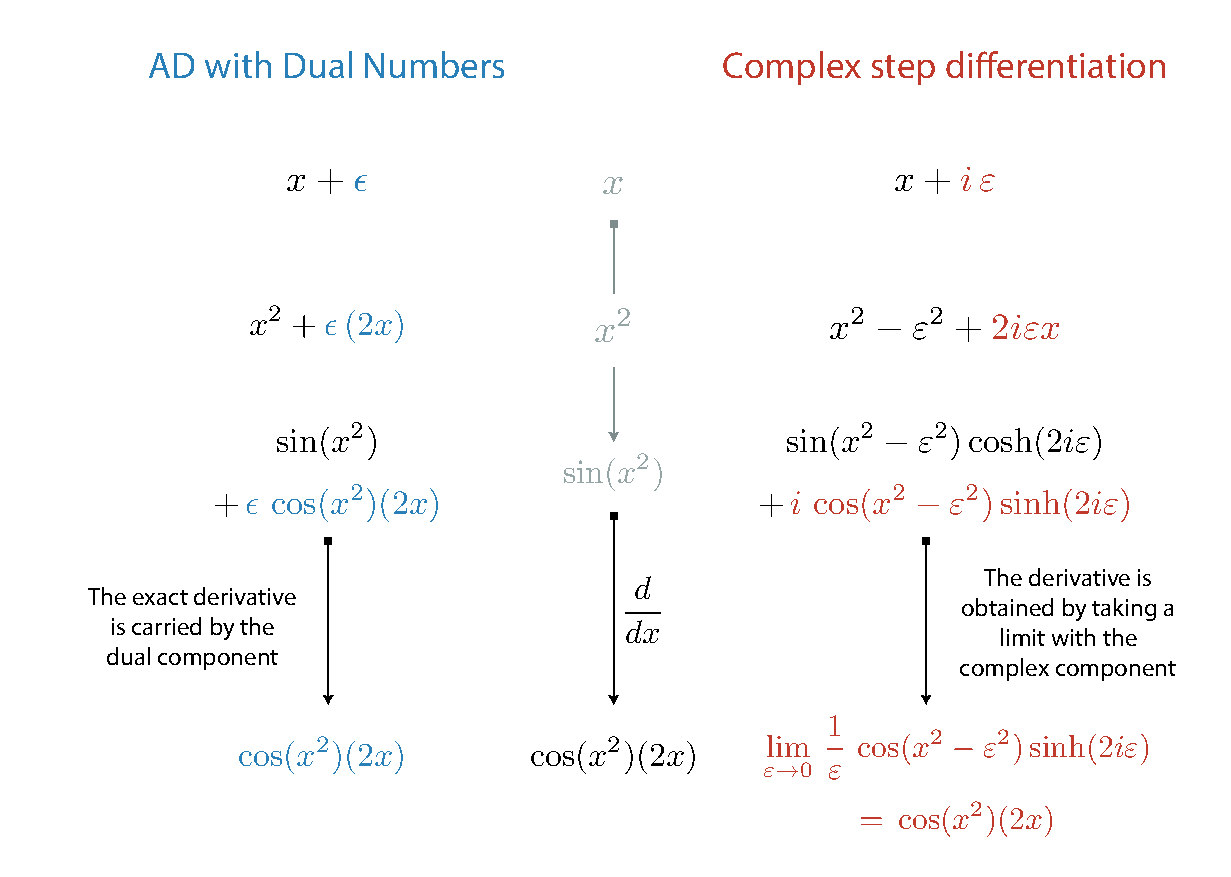
\includegraphics[width=0.75\textwidth]{figures/complex-step-AD.pdf}
    \caption{Comparison between AD implemented with dual numbers and complex step differentiation. For the simple case of the function $f(x) = \sin(x^2)$, we can see how each operation is carried in the forward step by the dual component (blue) and the complex component (red). Whereas AD gives the exact gradient at the end of the forward run, in the case of the complex step method we need to take the limit in the imaginary part. }
    \label{fig:complex-step-AD}
\end{figure}

\subsubsection{AD and symbolic differentiation with sparsity}

When sparsity patterns of the gradient/Jacobian to be computed are known, symbolic differentiation can be more efficient than AD \cite{Lantoine_Russell_Dargent_2012}.
In Section \ref{sec:vjp-jvp} we discussed how colored AD can be used to efficiently compute a sparse Jacobian.
However, colored AD has the limitation that an extremely sparse matrix can have no rows or columns independent of each other. 
Consider the arrowhead matrix given by
\begin{equation}
    J_{\text{arrowhead}} = \begin{bmatrix}
        j_{11} & j_{12}   & j_{13} & j_{14}     & j_{15}   \\
        j_{21} & j_{22}   &  0       & 0        & 0        \\
        j_{31} & 0        & j_{33}   & 0        & 0        \\
        j_{41} & 0        & 0        & j_{44}   & 0        \\
        j_{51} & 0        & 0        & 0        & j_{55}
    \end{bmatrix}.
\end{equation}
In this case, both reverse mode AD and forward mode AD will have to perform $n$ VJPs and JVPs, respectively (for $J_{\text{arrowhead}} \in \R^{n \times n}$ arrowhead matrix), and there is no computational benefit of coloring the matrix here. 
Instead, symbolic differentiation constructs a symbolic representation of the sparse Jacobian and can fill the Jacobian with $n + 2 \cdot (n-1)$ computations, where each computation is significantly cheaper than each VJP or JVP. 
Notice that for the arrowhead matrix example, a combination of forward and reverse AD can be used to color the Jacobian with two forward and one reverse AD evaluations. 
% This may be worth adding, but not sure yet.
% Consider the example given in \cite{Griewank:2008kh}
% \begin{equation}
%     L(x) = \ln \Psi_0 = \ln \sum_{i=1}^d w_i \Psi_i (e^{z_i \sin (x)}) 
% \end{equation}
% with $0 \geq w_i$ and $z_i \in \R$ some coefficients and $\Psi_i : \R \mapsto \R_{\geq 0}$. 
% Computer algebra systems are able to handle the common sub-expression $\cos(x) / \Psi_0 $ in $L'(x)$ to reduce the total number of multiplication involved in the derivative with respect to both forward and reverse AD, which instead will evaluate the sub-product with respect to the term   $\cos(x) / \Psi_0$.

\subsubsection{Discrete adjoints and reverse AD}
\label{section:comparison-discrete-adjoint-AD}

Both discrete adjoint methods and reverse AD are classified as discrete and reverse methods (see Figure \ref{fig:scheme-all-methods}). 
Furthermore, both methods introduce an intermediate adjoint associated with the partial derivative of the loss function (output variable) with respect to intermediate variables of the forward computation.
In the case of reverse AD, this adjoint is defined with the notation $\bar w$ (Equation \eqref{eq:reverse-mode-ad-definition}), while in the discrete adjoint method this correspond to each one of the variables $\lambda_1, \lambda_2, \ldots, \lambda_N$ (Equation \eqref{eq:linea-adjoint-state-equation}).
In this section we show that both methods are mathematically equivalent \cite{Zhu_Xu_Darve_Beroza_2021, li2020coupled}, but naive implementations using reverse AD can result in sub-optimal performances compared to the one obtained by directly employing the discrete adjoint method \cite{Alexe_Sandu_2009}. 

In order to have a better idea of how this works in the case of a numerical solver, let us consider again the case of a one-step explicit method, not necessarily linear, where the updates $u_{i}$ satisfy the equation $u_{i+1} = g_{i}(u_{i}, \theta)$.
Following the same schematics as in Figure \ref{fig:discrete-adjoint}, we represent the computational graph of the numerical method using the intermediate variables $g_1, g_2, \ldots, g_{N-1}$.
The dual/adjoint variables defined in reverse AD in this computational graph are given by 
\begin{equation}
    \bar g_i
    = 
    \frac{\partial u_{i+1}}{\partial g_i} \bar u_{i+1}
    = 
    \frac{\partial L}{\partial u_{i+1}} 
    +
    \frac{\partial g_{i+1}}{\partial u_i} \bar g_{i+1}.
\end{equation}
The updates of $\bar g_i$ then mathematically coincide with the updates in reverse mode of the adjoint variable $\lambda_i$ (see Equation \eqref{eq:adjoint-discrete-linear-example}).

\begin{figure}[t]
    \centering
    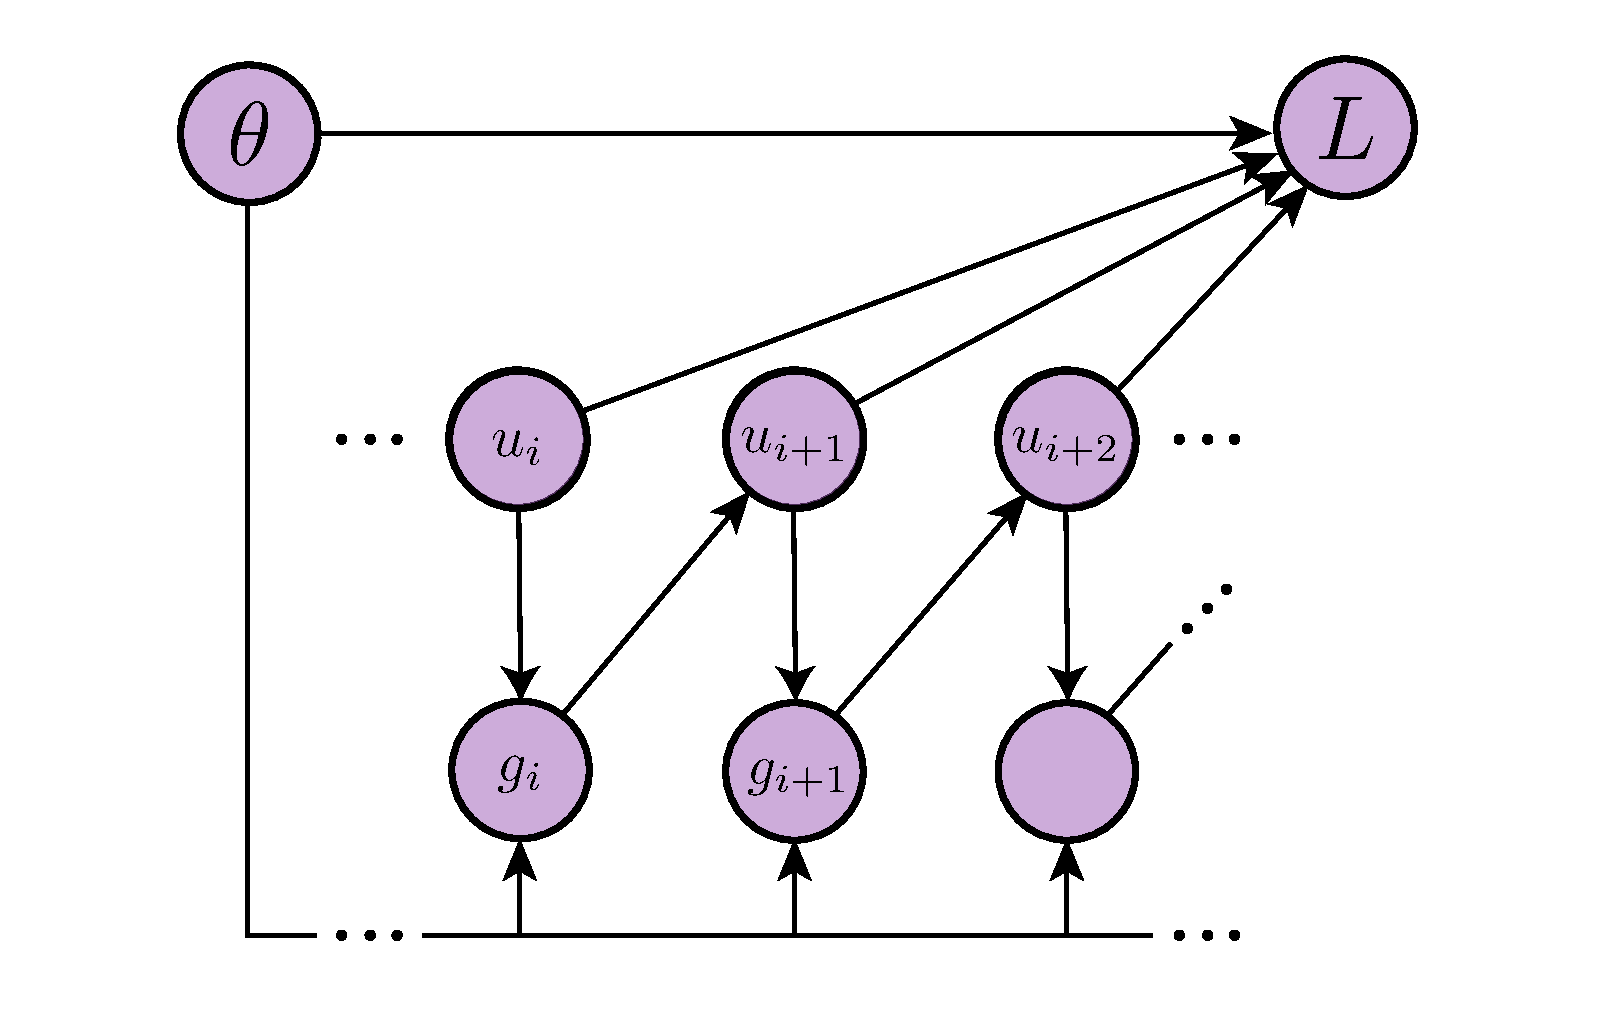
\includegraphics[width=0.65\textwidth]{figures/AD-discrete-adjoint.pdf}
    \caption{Computational graph associated to the discrete adjoint method. Reverse AD applied on top of the computational graph leads to the update rules for the discrete adjoint. The adjoint variable $\lambda_i$ in the discrete adjoint method coincides with the adjoint variable $\bar g_i$ defined in the backpropagation step.}
    \label{fig:ad-vs-discrete-adjoint}
\end{figure}

Modern numerical solvers use functions $g_i$ that correspond to nested functions, meaning $g_i = g_i^{(k_i)} \circ g_i^{(k_i-1)} \circ \ldots \circ g_i^{(1)} $. 
% When in an explicit solver this happens? 
This is certainly the case for implicit methods when $u_{i+1}$ is the solution of an iterative Newton method \cite{SUNDIALS-hindmarsh2005sundials}; or in cases where the numerical solver includes internal iterative sub-routines \cite{Alexe_Sandu_2009}.
If the number of intermediate function is large, reverse AD will result in a large computational graph, potentially leading to excessive memory usage and slow computation \cite{Margossian_2018, Alexe_Sandu_2009}.
A solution to this problem is to introduce a customized \textit{super node} that directly encapsulates the contribution to the full adjoint in $g_i$ without computing the adjoint for each intermediate function $g_i^{(j)}$.
Provided with the value of the Jacobian matrices $\frac{\partial g_i}{\partial u_i}$ and $\frac{\partial g_i}{\partial \theta}$, we can use the implicit function theorem to find 
the $\frac{\partial u_i}{\partial \theta}$ as the solution of the linear system of equations
\begin{equation}
    \frac{\partial g_i}{\partial u_i} \frac{\partial u_i}{\partial \theta} = -\frac{\partial g_i}{\partial \theta}
\end{equation}
and implement AD by directly solving this new system of equations \cite{christianson1994reverse, christianson1998reverse, Bell_Burke_2008}. 
% (this is equivalent to Equation \eqref{eq:adjoint-inversion-implicit-theorem})
In both cases, the discrete adjoint method can be implemented directly on top of a reverse AD tool that allows customized adjoint calculation \cite{rackauckas2021generalized}. 
% Furthermore, notice that instead of the full Jacobian, reverse methods only required to compute VJPs. 

% The code generated by AD is usually sub-optimal compared to the one define by the adjoint method \cite{Alexe_Sandu_2009}.
% Furthermore, implementation of black-box AD in the numerical solver with result in the differentiation of iterations and sub-routines inside the numerical solver \cite{Alexe_Sandu_2009}. 

\subsubsection{Consistency: forward AD and forward sensitivity equations}
\label{section:forwardAD-sensitivity}

The forward sensitivity equations can also be solved in discrete forward mode by numerically discretizing the original ODE and later deriving the discrete forward sensitivity equations \cite{ma2021comparison}. 
For most cases, this leads to the same result as in the continuous case \cite{FATODE2014}.
% To illustrate this, consider the simple forward Euler method applied to the original ODE given by $u_{t+1} = u_t + \Delta t \, f(u_t, \theta, t)$.
We can numerically solve for the sensitivity $s$ by extending the parameter $\theta$ to a multidimensional dual number %\cite{Neuenhofen_2018, RevelsLubinPapamarkou2016}, 
\begin{equation}
    \theta =
    \begin{bmatrix}
    \theta_1 \\
    \theta_2 \\
    \vdots \\
    \theta_p
    \end{bmatrix}
    \longrightarrow
    \begin{bmatrix}
    \theta_1 + \epsilon_1 \\
    \theta_2 + \epsilon_2 \\
    \vdots \\
    \theta_p + \epsilon_p
    \end{bmatrix}
\end{equation}
where $\epsilon_i \epsilon_j = 0$ for all pairs of $i$ and $j$ (see Section \ref{section:dual-numbers}). 
The dependency of the solution $u$ of the ODE on the parameter $\theta$ is now expanded following Equation \eqref{eq:dual-number-function} as 
\begin{equation}
    u =
    \begin{bmatrix}
    u_1 \\
    u_2 \\
    \vdots \\
    u_n
    \end{bmatrix}
    \longrightarrow
    \begin{bmatrix}
    u_1 + \sum_{j=1}^p \frac{\partial u_1}{\partial \theta_j} \epsilon_j \\
    u_2 + \sum_{j=1}^p \frac{\partial u_2}{\partial \theta_j} \epsilon_j \\
    \vdots \\
    u_p + \sum_{j=1}^p \frac{\partial u_n}{\partial \theta_j} \epsilon_j
    \end{bmatrix}
    = 
    u \, + \, s \, 
    \begin{bmatrix}
    \epsilon_1 \\
    \epsilon_2 \\
    \vdots \\
    \epsilon_p
    \end{bmatrix},
\end{equation}
that is, the dual component of the vector $u$ corresponds exactly to the sensitivity matrix $s$. 
This implies forward AD applied to any multistep linear solver will result in the application of the same solver to the forward sensitivity equation (Equation \eqref{eq:sensitivity_equations}).  
For example, for the forward Euler method this gives 
\begin{align}
\begin{split}
    u^{t+1} + s^{t+1} \, \epsilon 
    &= 
    u^t +  s^t \, \epsilon + \Delta t \, f (u^t + s^t \, \epsilon, \theta + \epsilon, t) \\
    &= 
    u^t + f(u^t, \theta, t) 
    + 
    \Delta t 
    \left( 
    \frac{\partial f}{\partial u} s^t + 
    \frac{\partial f}{\partial \theta}
    \right) \epsilon.
\end{split}
\label{eq:sensitivity-equation-AD}
\end{align}
The dual component corresponds to the forward Euler discretization of the forward sensitivity equation, with $s^t$ the temporal discretization of the sensitivity $s(t)$.

The consistency result for discrete and continuous methods also holds for Runge-Kutta methods \cite{Walther_2007}. 
When introducing dual numbers, the Runge-Kutta scheme in Equation \eqref{eq:Runge-Kutta-scheme} gives the following identities
\begin{align}
    u^{n+1} + s^{n+1} \epsilon 
    &= 
    s_n + \Delta t_n \sum_{i=1}^s b_i \dot k_i
    \\
    k_i + \dot k_i \epsilon
    &= 
    f \left(u^n + \sum_{j=1}^s a_{ij} k_j + \left( s^n + \sum_{j=1}^s a_{ij} \dot k_j \right) \epsilon , \theta + \epsilon ,  t_n + c_i \Delta t_n \right) \label{eq:rk-sensitivity-2}
\end{align}
with $\dot k_i$ the dual variable associated to $k_i$.
The partial component in Equation \eqref{eq:rk-sensitivity-2} carrying the coefficient $\epsilon$ gives 
\begin{align}
\begin{split}
    \dot k_i
    &= 
    \frac{\partial f}{\partial u} 
    \left(u^n + \sum_{j=1}^s a_{ij} k_j, \theta,  t_n + c_i \Delta t_n \right)
    \left( s^n + \sum_{j=1}^s a_{ij} \dot k_j \right) \\
    &+ 
    \frac{\partial f}{\partial \theta} 
    \left(u^n + \sum_{j=1}^s a_{ij} k_j, \theta,  t_n + c_i \Delta t_n \right),
\end{split}
\end{align}
which coincides with the Runge-Kutta scheme we would obtain for the original forward sensitivity equation. 
This means that forward AD on Runge-Kutta methods leads to solutions for the sensitivity that have the same convergence properties of the forward solver. 

Note that consistency does not imply that an ODE solver is necessarily correct or stable under such a transformation. 
Consistency of the adjoint may involve other aspects of the solver, such as adaptivity and error control. 
In Appendix \ref{appendix:dual-number-solver}, we demonstrate that common implementations of adaptive ODE solvers may not compute the right gradient when forward AD is applied to solver even though the process is mathematically consistent. 
This highlights that additional factors beyond consistency must be considered when investigating whether an implementation is convergent.

\subsubsection{Consistency: discrete and continuous adjoints}

% There is a large family of adjoint methods that in first order can be classified as discrete and continuous adjoints. 
As previously mentioned, the difference between the discrete and continuous adjoint methods is that the former follows the discretize-then-differentiate approach (also known as finite difference of adjoints \cite{Sirkes_Tziperman_1997}).
In contrast, continuous adjoint equations are derived analytically, without a priori consideration of the numerical scheme used to solve it. 
In some sense, we can think of the discrete adjoint $\lambda = (\lambda_1, \lambda_2, \ldots, \lambda_N)$ in Equation \eqref{eq:linea-adjoint-state-equation} as the discretization of the continuous adjoint $\lambda(t)$. 


A natural question then is if these two methods effectively compute the same gradient, i.e., if the discrete adjoint consistently approximate its continuous counterpart. 
Furthermore, since the continuous adjoint method requires to numerically solve the adjoint, we are interested in the relative accuracy of the forward and reverse step. 
It has been shown that for both explicit and implicit Runge-Kutta methods, as long as the coefficients in the numerical scheme given in Equation \eqref{eq:Runge-Kutta-scheme} satisfy the condition $b_i \neq 0$ for all $i=1,2, \ldots, s$, then the discrete adjoint is a consistent estimate of the continuous adjoint with same level of convergence as for the forward numerical solver \cite{Hager_2000,Walther_2007, sandu2006properties, sandu2011solution}.
To guarantee the same order of convergence, it is important that both the forward and backward solver use the same Runge-Kutta coefficients \cite{Alexe_Sandu_2009}.
Importantly, even when consistent, the code generated using the discrete adjoint using AD tools (see Section \ref{section:comparison-discrete-adjoint-AD}) can be sub-optimal and manual modification of the differentiation code are required to guarantee correctness \cite{Eberhard_Bischof_1996, alexe2007denserks}.

% For multilinear solver, ... 



